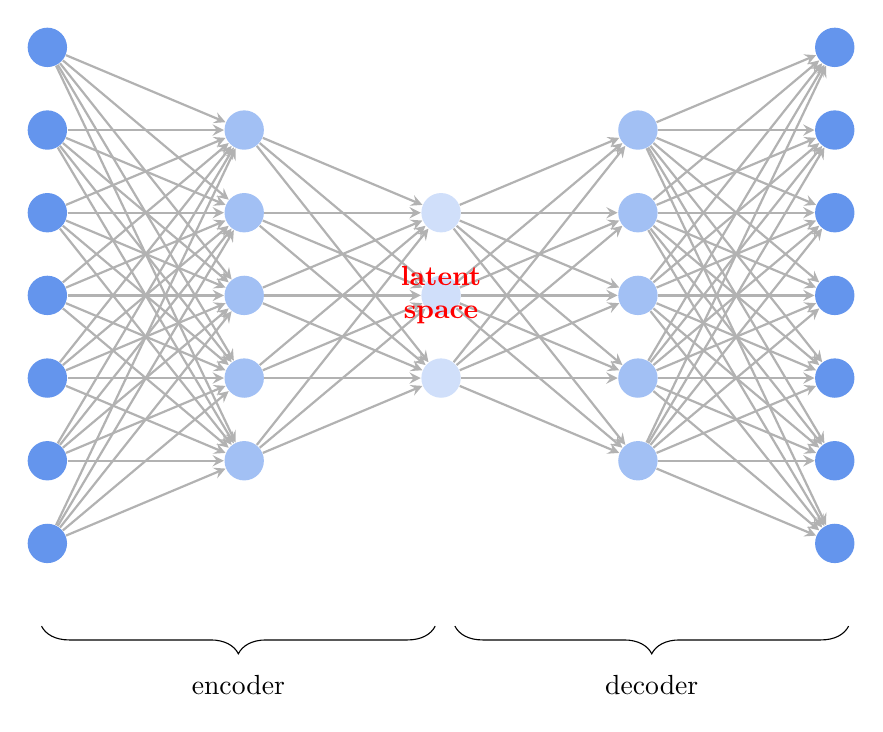
\begin{tikzpicture}[x=2.5cm, y=1.5cm,
	neuron/.style={circle, minimum size=0.5cm, inner sep = 0mm},
	weight/.style={font=\small, midway, fill=white, inner sep=1pt},
	>=stealth]
	
	% Neuronenzahlen
	\def\none{7}
	\def\ntwo{5}
	\def\nthree{3}
	\def\nfour{5}
    \def\nfive{7}
	
	% Schichtpositionen
	\def\xspace{0}
	
	% Eingabeschicht
	\foreach \y in {1, ..., \none}
	   \node[neuron, fill = CornflowerBlue] (A\y) at (0, -0.7*\y) {};

    \foreach \y in {1, ..., \ntwo}
	   \node[neuron, fill = CornflowerBlue!60] (B\y) at (1, -0.7*\y-0.7) {};

    \foreach \y in {1, ..., \nthree}
	   \node[neuron, fill = CornflowerBlue!30] (C\y) at (2, -0.7*\y-1.4) {};

    \foreach \y in {1, ..., \nfour}
	   \node[neuron, fill = CornflowerBlue!60] (D\y) at (3, -0.7*\y-0.7) {};

    \foreach \y in {1, ..., \nfive}
	   \node[neuron, fill = CornflowerBlue] (E\y) at (4, -0.7*\y) {};
	
    \foreach \d in {1, 2, ..., \none} {
        \foreach \s in {1, 2, ..., \ntwo} {
            \draw[->, thick, gray!60] (A\d) -- (B\s);
        }
    }

    \foreach \d in {1, 2, ..., \ntwo} {
        \foreach \s in {1, 2, ..., \nthree} {
            \draw[->, thick, gray!60] (B\d) -- (C\s);
        }
    }

    \foreach \d in {1, 2, ..., \nthree} {
        \foreach \s in {1, 2, ..., \nfour} {
            \draw[->, thick, gray!60] (C\d) -- (D\s);
        }
    }

    \foreach \d in {1, 2, ..., \nfour} {
        \foreach \s in {1, 2, ..., \nfive} {
            \draw[->, thick, gray!60] (D\d) -- (E\s);
        }
    }

    \draw [decorate,decoration={brace,amplitude=10pt},xshift=5pt]
    (1.9, -5.6) -- (-0.1, -5.6) node [midway,below=0.5cm] {encoder};

    \draw [decorate,decoration={brace,amplitude=10pt},xshift=5pt]
    (4, -5.6) -- (2, -5.6) node [midway,below=0.5cm] {decoder};

    \node[color = red, align = center] (txt) at (2, -4*0.7) {\textbf{latent}\\\textbf{space}};
	
\end{tikzpicture}
